\section{Auswertung}
Nachfolgend werden die gewonnen Messergebnisse dargestellt und nötige Rechnungen durchgeführt.
Zur Auswertung der AFM Aufnahmen wird die Software \textit{Gwyddion} verwendet.

\FloatBarrier
\subsection{Vermessung der Nanostruktur}

Zur Umrechnung zwischen Spannung am Piezo und Auslenkung wird nachfolgend der Faktor
$\SI{155}{\nano\meter \per \volt}$ benutzt.
Das aufgenommene Bild der Linienstruktur ist in Abbildung~\ref{fig: linien_profil}(a) dargestellt. Hieraus wurde
das Profil in Abbildung~(b) entnommen. Das Bild und auch das Profil zeigen deutlich einen gemessenen
Höhengradienten entlang beider Scan Richtungen. Zur Vermessung der Nanostruktur und auch zur Quantifizierung
dieses Höhengradienten wird wie folgt vorgegangen. Die Daten des Höhenprofils werden gemäß der
eingezeichneten vertikalen Linien in~\ref{fig: linien_profil}(b) jeweils dem oberen und unterem
Niveau der Struktur zugeordnet. Es werden nur Datenpunkte außerhalb der grau hinterlegten Bereiche verwendet.
Für beide Niveaus kann dann eine lineare Regression berechnet werden.
Die Steigungen beträgt in beiden Fällen ca. $\SI{10}{\nano\meter\per\micro\meter}$. Die Differenz
der Ordinatenabschnitte und damit die Höhe $h$ der Struktur ergibt sich zu
\begin{equation}
  h\ua{Linie} = \SI{0.113(5)}{\micro\meter}
\end{equation}
und weicht damit um ca. $\SI{13}{\percent}$ von der Herstellerangabe ($\SI{0.1}{\micro\meter}$) ab. Aus den Abständen der eingezeichneten
Linien in~\ref{fig: linien_profil}(b) kann der Strukturabstand $s$ zu
\begin{equation}
  s\ua{Linien} = \SI{5.03(9)}{\micro\meter}
\end{equation}
bestimmt werden, was einer Abweichung von etwa $\SI{0.6}{\percent}$ zur Angabe $\SI{5}{\micro\meter}$ entspricht.
\begin{figure}
  \centering
  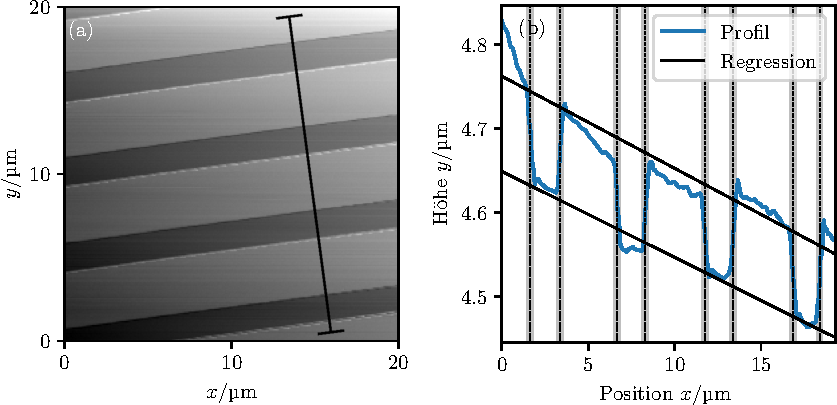
\includegraphics[scale = 1]{../analysis/data/nanostruktur_linien/linien_profil.pdf}
  \caption{Ergebnis der Messung an dem Linienprofil der Nanostruktur. (a) AFM Aufnahme mit eingezeichneten
  Linien, enlang derer das Profil in Abbildung (b) aufgenommen wurden. Das Profil ist
  über die Breite der in (a) eigezeichneten Balken gemittelt. Zudem sind in (b) die linearen Regressionen
  an die Datenpunkte eingezeichnet, die dem oberen bzw. unterem Niveau der Nanostruktur zugeordnet wurden.}
  \label{fig: linien_profil}
\end{figure}

Analog wird für die Quadratstruktur vorgegangen. Das AFM Bild, sowie ein horizontales und vertikales Profil sind
in Abbildung~\ref{fig: quadrate_profil} einzusehen. Es zeigt sich ein deutlicher Unterschied zwischen den Profilen.
Da das vertikale Profil (c) wesentlich stärker verrauscht ist, kann von einer schlechteren Auflösung des Systems
entlang der $y$-Richtung ausgegangen werden. Dies könnte an der Hysterese des zugehörigen Piezos liegen oder an
einer asymmetrischen Cantilever-Spitze. Da die fehlerhafte Messung der Struktur insbesondere an den Stufen der Struktur
auftritt, wird im Fall der vertikalen Linien ein größerer Bereich der Daten nicht verwendet (siehe
Abbildung~\ref{fig: quadrate_profil} (c)). Die gemessene Steigung des horizontalen Profils beträgt ca.
$\SI{8}{\nano\meter\per\micro\meter}$, die des vertikalen Profils ca. $\SI{5}{\nano\meter\per\micro\meter}$.
Aus dem horizontalen Profil ergibt sich für Strukturabstand und Höhe:
\begin{equation}
  h\ua{Quadrate} = \SI{0.1013(6)}{\micro\meter}, \quad s\ua{Quadrate} = \SI{9.62(9)}{\micro\meter}.
\end{equation}
Aus dem vertikalen Profil:
\begin{equation}
  h\ua{Quadrate} = \SI{0.0970(9)}{\micro\meter}, \quad s\ua{Quadrate} = \SI{10.004(9)}{\micro\meter}.
\end{equation}
Es ist somit zu beobachten, dass die gemessene Höhe und der Strukturabstand anhand des vertikalen Profils mit einer
Abweichung von $3$ bzw. $\SI{4}{\percent}$ näher an den Herstellerangaben liegen. Dies spricht dafür, dass
die Umrechnung zwischen Piezospannung und Verschiebungsstrecke, für $x$-(etwa entlang horizontalem Profil) und $y$-Richtung (etwa
entlang vertikalem Profil) unterschiedlich sind oder dass asymmetrische thermische Drifts und andere Störeinflüsse auftreten.
\begin{figure}
  \centering
  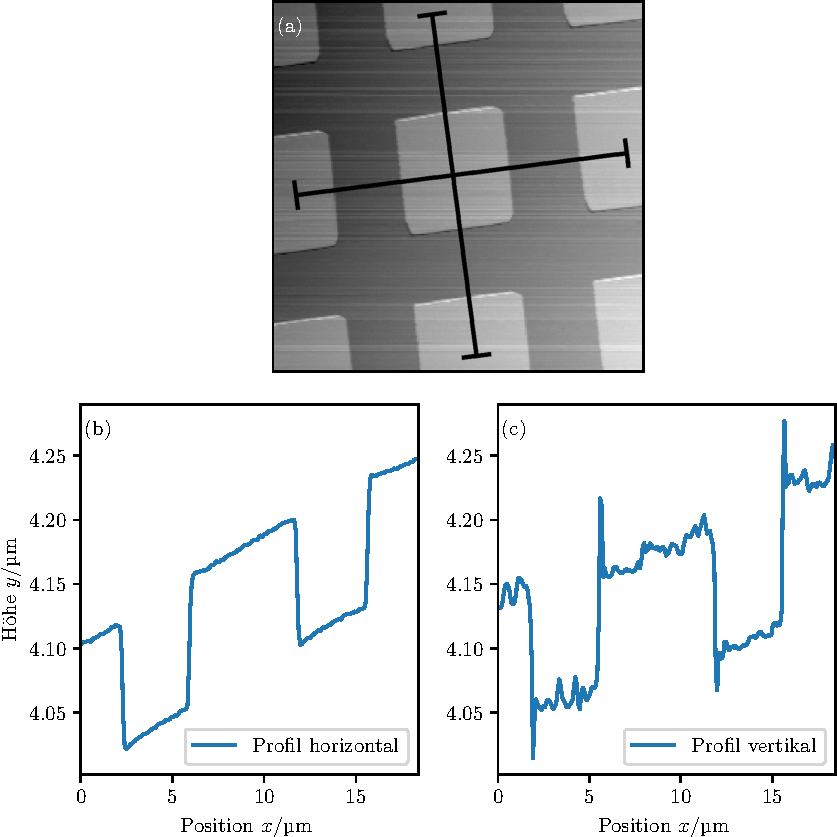
\includegraphics[scale = 1]{../analysis/data/nanostruktur_quadrate/quadrate_profile.pdf}
  \caption{Ergebnis der Messung an den quadratischen Nanostrukturen. (a) AFM Aufnahme mit eingezeichneten
  Linien, enlang derer die Profile in Abbildung (b) und (c) aufgenommen wurden. Die Profile sind
  über die Breite der in (a) eigezeichneten Balken gemittelt.}
  \label{fig: quadrate_profil}
\end{figure}

Das Ergebnis der Messung an den Kreisstrukturen ist in Abbildung~\ref{fig: kreise_profil} dargestellt. In Teil (b)
ist eine Aufnahme ohne Strain Gauge zu sehen. Der Vergleich mit Abbildungsteil (a) zeigt den Einfluss der Strain Gauge Funktion.
Die ersichtliche Verzerrung der Kreise wird verringert und ebenfalls der Kontrast erhöht. Dennoch bleibt auch mit eingeschalteter
Strain Gauge Funktion eine Verzerrung der Kreise zurück. Mittels zwei Profilen, die ebenfalls in~Abbildung~\ref{fig: kreise_profil}
gezeigt sind, können erneut die Abmessungen der Struktur ermittelt werden. Aus dem horizontalem Profil:
\begin{equation}
  h\ua{Kreise} = \SI{0.094(2)}{\micro\meter}, \quad s\ua{Kreise} = \SI{4.85(7)}{\micro\meter}.
\end{equation}
Aus dem vertikalen Profil:
\begin{equation}
  h\ua{Kreise} = \SI{0.090(3)}{\micro\meter}, \quad s\ua{Kreise} = \SI{5.06(6)}{\micro\meter}.
\end{equation}
Die Strukturgröße ist entlang der $y$-Richtung erneut näher an der Herstellerangabe $\SI{5}{\micro\meter}$.
Es zeigt sich zudem wieder eine stärkere Verzerrung der Daten entlang der $y$-Verschiebung.

\begin{figure}
  \centering
  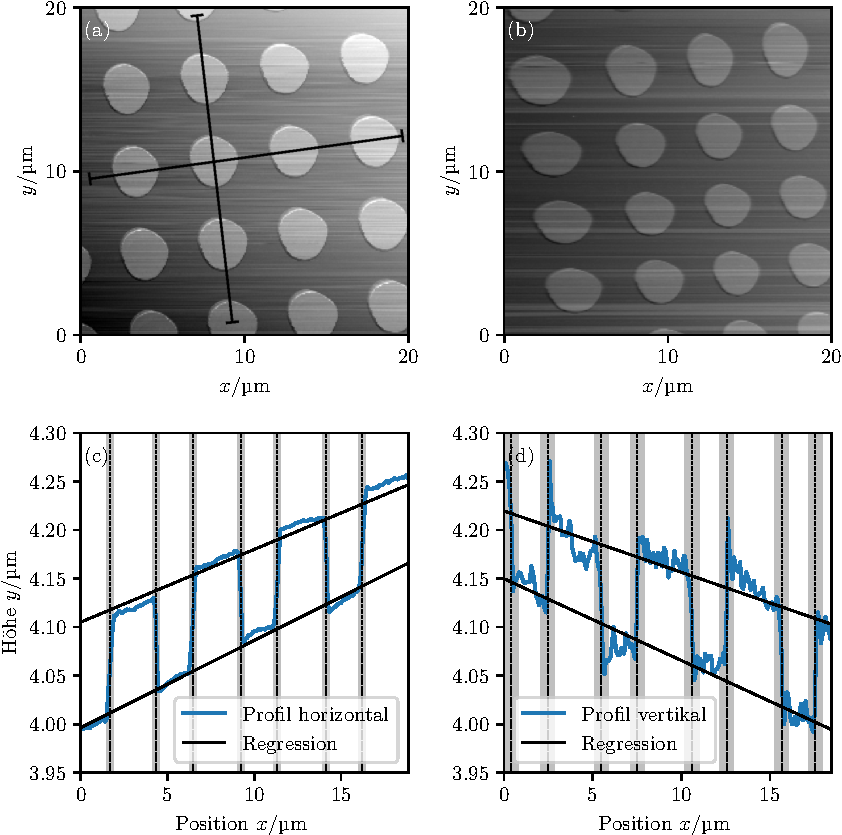
\includegraphics[scale = 1]{../analysis/data/nanostruktur_kreise/kreise_profile.pdf}
  \caption{(a) AFM Aufnahme der Kreiststruktur mit eingezeichneten Profilen, die in (c) und (d) aufgetragen sind.
    (b) zeigt eine Aufnahme mit ausgeschalteter Strain Gauge Kontrolle.}
  \label{fig: kreise_profil}
\end{figure}

\FloatBarrier
\subsection{Vermessung CD / DVD}
Die aufgenommenen AFM Bilder der CD und DVD Oberflächen sind in Abbildung~\ref{fig: cd} einzusehen.
Die Aufnahmen verfügen über einen schwachen Kontrast und eine schlechte Auflösung. Von einer
quantitativen Analyse der DVD Abmessungen wird daher abgesehen. Die vorhandene Blue-Ray
konnte mit dem Aufbau nicht analysiert werden.

In Abbildung~\ref{fig: cd} (a) sind die Linien eingezeichnet, entlang derer die relevanten Abmessungen der
CD Struktur mit Gwyddion ausgemessen wurden. Aus dem Profil in Abbildung~\ref{fig: cd} (b) kann die
Strukturhöhe zu etwa $\SI{0.07}{\micro\meter}$ ermittelt werden. Das Auslesen der Infomation auf einer
CD erfolgt über Interferenzeffekte. Die Pittiefe ist so gewählt, dass sich der Laufweg des Lichts
um eine halbe Wellenlänge ändert, wenn ein Pit vorliegt. Im Falle von CDs wird ein Laser mit $\SI{780}{\nano\meter}$
verwendet, dessen Wellenlänge im Medium etwa $\SI{500}{\nano\meter}$ beträgt. Die optimale Pit-Tiefe wäre daher
$\SI{250}{\nano\meter}$ \cite{cd_theorie}. Der hier zu klein gemessene Wert, könnte durch eine zu grobe Spitze
bedingt sein.

Des weiteren ergeben sich folgende Abmessungen der Pits:
\begin{align}
  \begin{aligned}
    \text{Spurbreite: } &     &\approx  \SI{0.227}{\micro\meter}\\
    \text{Spurabstand: } &        &\approx \SI{1.533}{\micro\meter} \\
    \text{minimale Pitlänge: } &     &\approx \SI{0.485}{\micro\meter} \\
    \text{maximale Pitlänge: } &    &\approx \SI{1.622}{\micro\meter}.
  \end{aligned}
\end{align}
Hieraus kann die Speicherkapazität ermittelt werden. Eine CD hat in etwa eine Fläche von $\SI{100}{\centi\meter\squared}$. Mit dem Spurabstand
$\SI{1.53}{\micro\meter}$ ergibt sich daraus
eine Länge der Gesamtspur von $\SI{6.5}{\kilo\meter}$. Diese Länge geteilt durch die minimale Bitlänge $\SI{0.24}{\micro\meter}$
(halbe minimale Pitlänge) ergibt die Anzahl an Bits $\num{2.7e10}$.
Nun muss die \textit{Eight-to-Fourteen}
Methode beachtet werden um daraus die Speicherkapazität zu bestimmen:
\begin{equation}
  \text{CD Speicherkapazität: } \frac{\num{2.7e10}}{14 + 3} \approx \SI{1.6}{GB}.
\end{equation}
Die maximale Speicherkapazität von CDs beträgt gewöhnlich $\SI{900}{MB}$. Hierzu muss jedoch die innere Speicherstruktur einer CD beachtet werden, die dazu führt,
dass nicht die volle mögliche Speicherkapazität genutzt werden kann, welche hier bestimmt wurde. Zudem könnten zu klein gemessene Pitdimensionen
zu einem fehlerhaften Ergebnis führen. Bei der Vermessung der Quadrate wurden in $x$-Richtung bereits zu kleine Strukturwerte gemessen. Dies spricht dafür,
dass der hier gemessene Spurabstand zu klein ist. Dies führt zu einer erhöhten Speicherkapazität.

\begin{figure}
  \centering
  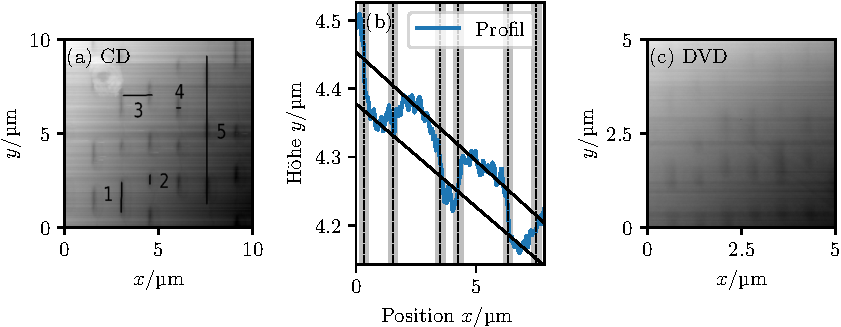
\includegraphics[scale = 1]{../analysis/data/cd/cd_profil.pdf}
  \caption{(a) AFM Aufnahme der CD mit eingezeichneten Längen: 1 maximale Pitlänge, 2 minimale Pitlänge,
  3 Spurabstand, 4 Spurbreite und 5 Profil, das in (b) gezeigt ist. (c) zeigt das Bild der DVD.}
  \label{fig: cd}
\end{figure}

\FloatBarrier
\subsection{Kraft-Abstands-Kurven}
Zur Berechnung der Kraft aus gemessenen Abständen, ist zunächst die Federkonstante des Cantilvers zu bestimmen. Diese kann
aus seiner Geometrie und Elastizität gemäß
\begin{equation}
  k = \frac{E \, b \, h^3}{4 \, l^3}
\end{equation}
berechnet werden. Mit der Höhe $h = \SI{2}{\micro\meter}$, Breite $b = \SI{50}{\micro\meter}$, Länge $l = \SI{450}{\micro\meter}$
des Cantilevers, die aus dem Datenblatt~\cite{cantilever} entnommen wurden, und dem Elastizitätsmodul von Silizium
$E = \SI{160}{\giga\pascal}$~\cite{emodulsi}
ergibt sich
\begin{equation}
  k = \SI{0.2}{\newton \per \meter}.
\end{equation}
Der Wert deckt sich mit Wert aus \cite{cantilever} und wird im Folgenden verwendet.

Abbildung~\ref{fig: force_distance} zeigt zum qualitativen Vergleich der drei aufgenommenen Kraft-Abstands-Kurven der Proben
Edelstahl, DLC und Teflon. Der Name Kraft-Abstands-Kurve wird verwendet, obwohl in den Plots die Differenzspannung der Photodiode
gegen das Spannungssignal des Piezos in $z$-Richtung aufgetragen ist. Die Spannung am Piezo wird, wie vom Hersteller in~\cite{afm_datasheet}
vorgeschlagen, mit dem Faktor $20 / 75 \si{\micro\meter\per\volt}$ in die Ausdehnung des Piezos umgerechnet.
Die Kurve von der Messung mit Edelstahl weicht im Maximalwert der Differenzspannung deutlich von den anderen beiden Kurven ab. Bei der
Teflon Kurve ist die Ruhelage weiter nach unten verschoben.
Im Fall der DLC Probe fällt auf, dass nach dem Pull-off eine Art Überschwingen
des Cantilevers über die Ruhelage stattfindet. Hiebei könnte es sich jedoch auch um wenige fehlerhafte Datenpunkte handeln.
Zur Diskussion des generellen Verlaufs einer solchen Kurve, ist in Abbildung~\ref{fig: force_distance_teflon} die Kurve
für Teflon vergrößert dargestellt und die relevanten Punkte und Bereiche beschriftet.
\begin{figure}
  \centering
  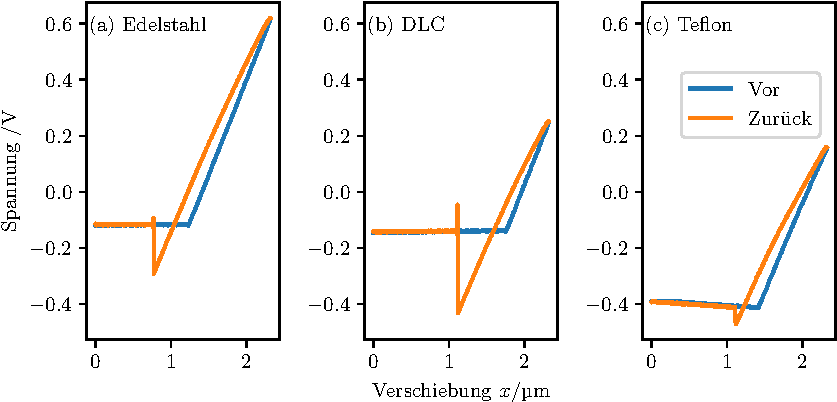
\includegraphics[scale = 1]{../analysis/data/force_distance/force_distance.pdf}
  \caption{Vergleich der drei aufgenommenen Kraft-Distanz-Kurven von Edelstahl, DLC und Teflon.}
  \label{fig: force_distance}
\end{figure}
\begin{figure}
  \centering
  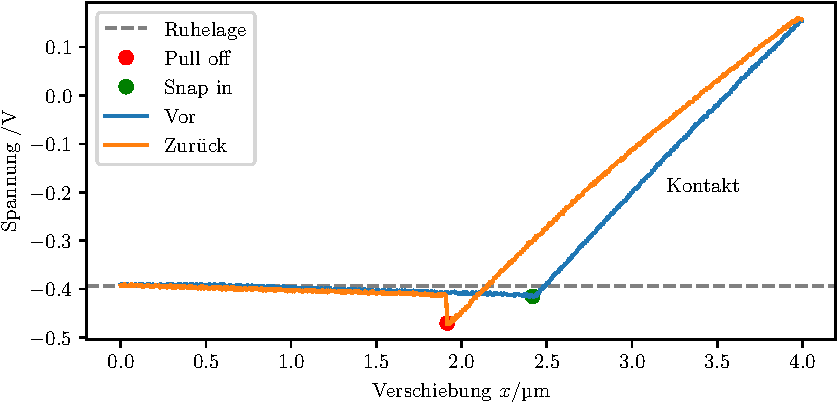
\includegraphics[scale = 1]{../analysis/data/force_distance/force_distance_teflon.pdf}
  \caption{Kraft-Abstands-Kurve von Teflon mit Markierungen.}
  \label{fig: force_distance_teflon}
\end{figure}
Der Pull-off Punkt ist deutlich zu erkennen, während der Snap-in nicht stark ausgeprägt ist. Hierfür wird
jeweils der Punkt vor dem Anstieg der Kurve beim Annähern von Spitze und Probe festgelegt. Zudem fällt auf, dass
die Kurve beim Entfernen von Spitze und Probe im Bereich des Kontaktes oberhalb verläuft. Dies ist auf die
Hysterese des Piezos zurückzuführen.

Zur Bestimmung des Elastizitätsmoduls von Teflon werden die Bereiche rechts von dem Snap-in betrachtet. Diese Daten aus den drei Kurven sind
in Abbildung~\ref{fig: depth} noch einmal aufgetragen, wobei der Ursprung jeweils in den Snap-in Punkt gelegt wurde. Die Daten sind
jeweils nur bis zu einem gemeinsamen maximalen Verschiebungspunkt gezeichnet.
Die beiden Kurven von Edelstahl und DLC überlagern sich gänzlich (siehe (c)), da beide Materialien undeformierbar sind.
Es ist deutlich zu erkennen, dass
die Steigung der Geraden von Teflon geringer ist als die von DLC und Edelstahl, was auf das Eindringen der Spitze in die Probe zurückzuführen ist.
Die Eindringtiefe am maximalen Verschiebungspunkt kann gewonnen werden, indem der horizontale Abstand der beiden Kurven in den Abbildungen~\ref{fig: depth}
(a) und (b) gemessen wird. Die Eindringtiefe $\delta$ entspricht dem Abstand der beiden eingezeichneten vertikalen Linien.
Es ergeben sich die Werte
\begin{equation}
  \text{(a): } \delta \approx \SI{0.13}{\micro\meter} \quad \text{und (b): }\delta \approx \SI{0.070}{\micro\meter}.
\end{equation}
Gemäß Formel~\eqref{eqn:emodul} kann daraus der Elastizitätsmodul $E$ gewonnen werden:
\begin{equation}
  \text{(a): } E \approx \SI{120}{\mega \pascal} \quad \text{und (b): } E \approx \SI{260}{\mega \pascal}.
\end{equation}
Die Werte weichen deutlich voneinander ab.
In Quelle~\cite{emodulteflon} ist der Wert
\begin{equation}
  E\ua{lit} = \SI{420}{\mega \pascal}
\end{equation}
zu finden. Die hier gemessenen Werte liegen also in der gleichen Größenordnung.

\begin{figure}
  \centering
  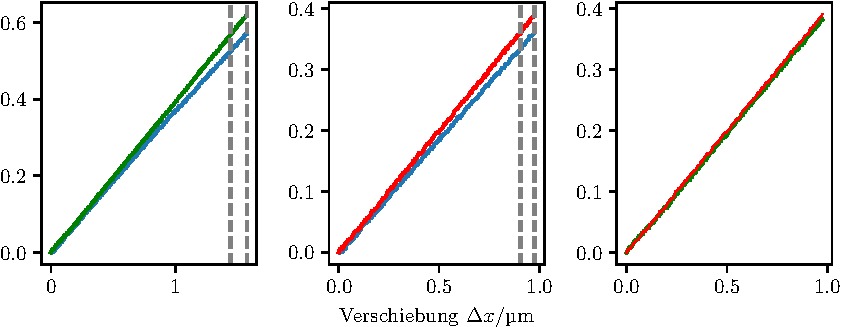
\includegraphics[scale = 1]{../analysis/data/force_distance/eindringtiefe.pdf}
  \caption{Vergleich der Kraft-Abstands-Kurven zur Bestimmung der Eindringtiefe des Cantilevers in die Teflon Probe.
  Es jeweils der lineare Kontaktbereich der Kraft-Abstands-Kurven dargestellt, wobei der Ursprung in den Snap-in Punkt
  gelegt wurde.}
  \label{fig: depth}
\end{figure}

Abschließend kann die maximal wirkende Adhäsionskraft bestimmt werden. Hierzu wird der horizontale
Abstand zwischen dem Pull-off und Snap-in mit der Federkonstante des Cantilevers multipliziert (gemäß des Hooke'schen Gesetzes).
Für die drei Proben ergeben sich die folgenden Werte:
\begin{align}
  \begin{aligned}
    \text{Edelstahl: } & F\ua{adh} &\approx \SI{157}{\nano\newton}\\
    \text{DLC: } & F\ua{adh}       &\approx \SI{219}{\nano\newton}\\
    \text{Teflon: } & F\ua{adh}    &\approx \SI{100}{\nano\newton}.
  \end{aligned}
\end{align}
Alle Werte liegen in der gleichen Größenordnung $\sim \SI{100}{\nano\newton}$. Äußere Einflüsse, wie vorherrschende Luftfeuchtigkeit
oder die Hysterese der Piezos können nicht quantifiziert werden. Da aber alle Werte mit der gleichen Spitze und in kurz aufeinander
folgenden Zeiten gemessen wurden, kann zumindest davon ausgegangen werden, dass die Messwerte vergleichbar sind. Es lässt sich also feststellen, dass die
Adhäsionskraft bei der DLC Probe am höchsten ist.
\FloatBarrier
